% Options for packages loaded elsewhere
\PassOptionsToPackage{unicode}{hyperref}
\PassOptionsToPackage{hyphens}{url}
\PassOptionsToPackage{dvipsnames,svgnames,x11names}{xcolor}
%
\documentclass[
  authoryear]{elsarticle}

\usepackage{amsmath,amssymb}
\usepackage{iftex}
\ifPDFTeX
  \usepackage[T1]{fontenc}
  \usepackage[utf8]{inputenc}
  \usepackage{textcomp} % provide euro and other symbols
\else % if luatex or xetex
  \usepackage{unicode-math}
  \defaultfontfeatures{Scale=MatchLowercase}
  \defaultfontfeatures[\rmfamily]{Ligatures=TeX,Scale=1}
\fi
\usepackage{lmodern}
\ifPDFTeX\else  
    % xetex/luatex font selection
\fi
% Use upquote if available, for straight quotes in verbatim environments
\IfFileExists{upquote.sty}{\usepackage{upquote}}{}
\IfFileExists{microtype.sty}{% use microtype if available
  \usepackage[]{microtype}
  \UseMicrotypeSet[protrusion]{basicmath} % disable protrusion for tt fonts
}{}
\makeatletter
\@ifundefined{KOMAClassName}{% if non-KOMA class
  \IfFileExists{parskip.sty}{%
    \usepackage{parskip}
  }{% else
    \setlength{\parindent}{0pt}
    \setlength{\parskip}{6pt plus 2pt minus 1pt}}
}{% if KOMA class
  \KOMAoptions{parskip=half}}
\makeatother
\usepackage{xcolor}
\setlength{\emergencystretch}{3em} % prevent overfull lines
\setcounter{secnumdepth}{5}
% Make \paragraph and \subparagraph free-standing
\ifx\paragraph\undefined\else
  \let\oldparagraph\paragraph
  \renewcommand{\paragraph}[1]{\oldparagraph{#1}\mbox{}}
\fi
\ifx\subparagraph\undefined\else
  \let\oldsubparagraph\subparagraph
  \renewcommand{\subparagraph}[1]{\oldsubparagraph{#1}\mbox{}}
\fi


\providecommand{\tightlist}{%
  \setlength{\itemsep}{0pt}\setlength{\parskip}{0pt}}\usepackage{longtable,booktabs,array}
\usepackage{calc} % for calculating minipage widths
% Correct order of tables after \paragraph or \subparagraph
\usepackage{etoolbox}
\makeatletter
\patchcmd\longtable{\par}{\if@noskipsec\mbox{}\fi\par}{}{}
\makeatother
% Allow footnotes in longtable head/foot
\IfFileExists{footnotehyper.sty}{\usepackage{footnotehyper}}{\usepackage{footnote}}
\makesavenoteenv{longtable}
\usepackage{graphicx}
\makeatletter
\def\maxwidth{\ifdim\Gin@nat@width>\linewidth\linewidth\else\Gin@nat@width\fi}
\def\maxheight{\ifdim\Gin@nat@height>\textheight\textheight\else\Gin@nat@height\fi}
\makeatother
% Scale images if necessary, so that they will not overflow the page
% margins by default, and it is still possible to overwrite the defaults
% using explicit options in \includegraphics[width, height, ...]{}
\setkeys{Gin}{width=\maxwidth,height=\maxheight,keepaspectratio}
% Set default figure placement to htbp
\makeatletter
\def\fps@figure{htbp}
\makeatother

\makeatletter
\@ifpackageloaded{caption}{}{\usepackage{caption}}
\AtBeginDocument{%
\ifdefined\contentsname
  \renewcommand*\contentsname{Table of contents}
\else
  \newcommand\contentsname{Table of contents}
\fi
\ifdefined\listfigurename
  \renewcommand*\listfigurename{List of Figures}
\else
  \newcommand\listfigurename{List of Figures}
\fi
\ifdefined\listtablename
  \renewcommand*\listtablename{List of Tables}
\else
  \newcommand\listtablename{List of Tables}
\fi
\ifdefined\figurename
  \renewcommand*\figurename{Figure}
\else
  \newcommand\figurename{Figure}
\fi
\ifdefined\tablename
  \renewcommand*\tablename{Table}
\else
  \newcommand\tablename{Table}
\fi
}
\@ifpackageloaded{float}{}{\usepackage{float}}
\floatstyle{ruled}
\@ifundefined{c@chapter}{\newfloat{codelisting}{h}{lop}}{\newfloat{codelisting}{h}{lop}[chapter]}
\floatname{codelisting}{Listing}
\newcommand*\listoflistings{\listof{codelisting}{List of Listings}}
\makeatother
\makeatletter
\makeatother
\makeatletter
\@ifpackageloaded{caption}{}{\usepackage{caption}}
\@ifpackageloaded{subcaption}{}{\usepackage{subcaption}}
\makeatother
\journal{JIMR}
\ifLuaTeX
  \usepackage{selnolig}  % disable illegal ligatures
\fi
\usepackage[]{natbib}
\bibliographystyle{elsarticle-harv}
\usepackage{bookmark}

\IfFileExists{xurl.sty}{\usepackage{xurl}}{} % add URL line breaks if available
\urlstyle{same} % disable monospaced font for URLs
\hypersetup{
  pdftitle={Conceptualizing open health data platforms for low- and middle income countries},
  pdfauthor={Daniel Kapitan; Femke Heddema; Julie Fleischer; Chris Ihure; Antragama Abbas; Steven Wanyee; XXX; John Grimes; Mark van der Graaf; Mark de Reuver},
  pdfkeywords={Analytics-on-FHIR, SQL-on-FHIR, HIE, data
platforms, LMICs, digital health},
  colorlinks=true,
  linkcolor={blue},
  filecolor={Maroon},
  citecolor={Blue},
  urlcolor={Blue},
  pdfcreator={LaTeX via pandoc}}

\setlength{\parindent}{6pt}
\begin{document}

\begin{frontmatter}
\title{Conceptualizing open health data platforms for low- and middle
income countries}
\author[1,2]{Daniel Kapitan%
%
}
 \ead{daniel@kapitan.net} 
\author[1]{Femke Heddema%
%
}

\author[1]{Julie Fleischer%
%
}

\author[3]{Chris Ihure%
%
}

\author[4]{Antragama Abbas%
%
}

\author[5]{Steven Wanyee%
%
}

\author[6]{XXX%
%
}

\author[7]{John Grimes%
%
}

\author[1]{Mark van der Graaf%
%
}

\author[4]{Mark de Reuver%
%
}


\affiliation[1]{organization={PharmAccess
Foundation},city={Amsterdam},country={the
Netherlands},countrysep={,},postcodesep={}}
\affiliation[2]{organization={Eindhoven University of
Technology},city={Eindhoven},country={the
Netherlands},countrysep={,},postcodesep={}}
\affiliation[3]{organization={PharmAccess
Kenya},city={Nairobi},country={Kenya},countrysep={,},postcodesep={}}
\affiliation[4]{organization={Delft University of
Technology},city={Delft},country={the
Netherlands},countrysep={,},postcodesep={}}
\affiliation[5]{organization={IntelliSOFT},city={Nairobi},country={Kenya},countrysep={,},postcodesep={}}
\affiliation[6]{organization={ONA},city={Nairobi},country={Kenya},countrysep={,},postcodesep={}}
\affiliation[7]{organization={Australian e-Health Research
Centre},city={Brisbane},country={Australia},countrysep={,},postcodesep={}}

\cortext[cor1]{Corresponding author}










        
\begin{abstract}
TO DO: add abstract.
\end{abstract}





\begin{keyword}
    Analytics-on-FHIR \sep SQL-on-FHIR \sep HIE \sep data
platforms \sep LMICs \sep 
    digital health
\end{keyword}
\end{frontmatter}
    
\section{Introduction}\label{sec-intro}

\subsection{The paradox of open for digital vs.~data platforms in
healthcare}\label{the-paradox-of-open-for-digital-vs.-data-platforms-in-healthcare}

It is a widely held belief that digital technologies have an important
role to play in strengthening health systems in low- and middle income
countries (LMICs), as exemplified by the WHO global strategy on digital
health \citep{who2021global}. The adoption rate of mobile phones in
LMICs has been an important driver in implementing digital health
solutions \citep{mccool2022mobile}. Yet, there are many shortcomings and
challenges, including the current fragmentation of digital platforms and
the lack of clear-cut pathways of scaling up digital health programmes,
such that they can support sustainable and equitable change of national
health systems in LMICs
\citep{mccool2022mobile, who2019recommendations, neumark2021digital}.

A commonly used perspective to scrutinize digital health is to consider
it as a digital platform \citep{dereuver2018digital}. Digital platforms
have disrupted many sectors but have just started to make inroads into
highly regulated industries such as healthcare \citep{ozalp2022digital}.
In this light, the challenges faced by LMICs in establishing national
digital health platforms have a lot in common with those faced by high
income countries. From a technological perspective, interoperability
issues, weak integrations, siloed data repositories and overall lack of
openness are often reported as key impediments
\citep{malm-nicolais2023exploring, mehl2023fullstac}. From a societal
perspective, issues pertaining to the winner-takes-all nature of digital
platforms are hotly debated as many jurisdictions make work to ensure
these new digital health platforms indeed serve the common good of
achieving universal health coverage \citep{sharon2018when}.

Case studies on digital platforms in healthcare point to an emerging
pattern where the focus shifts from the digital platform with its
defining software and hardware components, to the data as the primary
object of interest in and of itself
\citep{ozalp2022digital, alaimo2022organizations}. This observation ties
into the proposed research agenda by de Reuver et al.~to consider data
platforms as a phenomenon distinct from digital platforms
\citep{dereuver2022openness}. Generally, data platforms inherit the
characteristics of digital platforms. For example, the economic
perspective on digital platforms stresses their multi-sidedness with
developers and consumers, while data platforms are used by data owners,
data consumers and third party solution providers. At the same time,
data platforms differ as their main offerings revolve around data. From
a market perspective, data platforms have more moderate network effects
and are more susceptible to fragmentation and heterogeneity.

Particularly relevant in the context of health data platforms (HDPs), is
the conceptualization of openness. The shift in perspective from digital
platforms to data platforms coincides with the paradox of open
\citep{keller2021paradox}. Originally, openness of digital platforms
focused on open source, open standards and copyrights, which by has been
superseded by ``\ldots{} conflicts about privacy, economic value
extraction, the emergence of artificial intelligence, and the
destabilizing effects of dominant platforms on (democratic) societies.
Instead of access to information, the control of personal data has
emerged in the age of platforms as the critical contention.''
\citep{keller2021paradox}. These conflicts are particularly salient in
the healthcare domain, as is evidenced by the polemic surrounding data
spaces \citep{otto2022designing} and data solidarity
\citep{kickbusch2021lancet, prainsack2022data, prainsack2023beyond}.
Openness is particularly relevant if we are to realize a
solidarity-based approach to health data sharing that i) gives people a
greater control over their data as active decision makers; ii) ensures
that the value of data is harnessed for public good; and iii) moves
society towards equity and justice by counteracting dynamics of data
extraction \citep{prainsack2022data}.

\subsection{From health information exchanges to health data
platforms}\label{from-health-information-exchanges-to-health-data-platforms}

This paper is motivated by the conflation of a number of developments
relevant to the design and implementation of open, solidarity-based HDPs
in LMICs. First, the OpenHIE framework \citep{openhie} has been adopted
by many sub-Saharan African countries \citep{mamuye2022health} as the
architectural blueprint for implementing nation-wide health information
exchanges (HIE), including Nigeria \citep{dalhatu2023paper}, Kenya
\citep{thaiya2021adoption} and Tanzania \citep{nsaghurwe2021one}. These
countries have, as a matter of course, extended the framework to include
``analytics services'' as an additional domain. The rationale for this
addition is to facilitate secondary reuse of health data for academic
research, real-world evidence studies etc. which can be framed within
the context of ongoing efforts towards Findable, Accessible,
Interoperable and Reusable (FAIR) sharing of health data
\citep{guillot2023fair}. In doing so, however, we have implicitly moved
from conceptualizing digital health platforms (the original OpenHIE
specification) to health data platforms. This is problematic because the
notion of openness, which is assumed to be essential in establishing
solidarity-based approaches to data sharing, is inherently different for
a data platform compared to a digital platform.

Conceptually, the OpenHIE framework constitutes a framework for an open
digital platform. Openness for digital platforms refers to i) the use of
open boundary resources, that is, specifications for the various
healthcare specific workflows and information standards such as FHIR;
and ii) the use of open source components that are available as digital
public goods\citep{digitalpublicgoods}. If we are to use the OpenHIE
framework as an open data platform, we need to extend the standards,
technologies and architecture to include functionality for data sharing
and reuse. Distinguishing four types of data sharing
(Table~\ref{tbl-types-data-sharing}), the purpose of this paper is to
investigate how new standards and technologies that can establish
openness of HDPs can be integrated into the OpenHIE architecture
framework. The lack of detailed specifications and consensus of this
addition to OpenHIE currently stands in the way of development projects
that aim to establish HDPs in LMICs. In addition, we explicitly address
the requirement of downward scalability as we aim to implement health
data platforms in resource constrained setting of LMICs.

\begin{longtable}[]{@{}
  >{\centering\arraybackslash}p{(\columnwidth - 4\tabcolsep) * \real{0.1200}}
  >{\raggedright\arraybackslash}p{(\columnwidth - 4\tabcolsep) * \real{0.3200}}
  >{\raggedright\arraybackslash}p{(\columnwidth - 4\tabcolsep) * \real{0.5600}}@{}}
\caption{Types of data sharing and in relation to new standards and
technology enablers to create
openness.}\label{tbl-types-data-sharing}\tabularnewline
\toprule\noalign{}
\begin{minipage}[b]{\linewidth}\centering
\end{minipage} & \begin{minipage}[b]{\linewidth}\raggedright
\textbf{Type of data sharing}
\end{minipage} & \begin{minipage}[b]{\linewidth}\raggedright
\textbf{Technology enablers to create openness of health data platforms}
\end{minipage} \\
\midrule\noalign{}
\endfirsthead
\toprule\noalign{}
\begin{minipage}[b]{\linewidth}\centering
\end{minipage} & \begin{minipage}[b]{\linewidth}\raggedright
\textbf{Type of data sharing}
\end{minipage} & \begin{minipage}[b]{\linewidth}\raggedright
\textbf{Technology enablers to create openness of health data platforms}
\end{minipage} \\
\midrule\noalign{}
\endhead
\bottomrule\noalign{}
\endlastfoot
\textbf{1} & Data at the most granular (patient) level, which is
persisted and used to provide a longitudinal record. & \textbf{Bulk FHIR
API}: has by now been incorporated in all major FHIR implementations the
FHIR standard can be readily used to support data sharing to
patient-level data across a patient population
\citep{mandl2020push, jones2021landscape}. \\
\textbf{2} & Aggregated data, for example statistics for policy
evaluation and benchmarking & \textbf{SQL-on-FHIR specification}
\citep{sql-on-fhir}: provides a standardised approach to make FHIR work
well with familiar and efficient SQL engines that are most commonly used
in analytical workflows. Builds on FHIRPath \citep{hl72020fhirpath}
expressions in a logical structure to specify things like column names
and unnested items. Implementations of this approach are available or
forthcoming, including open source implementations such as Pathling
\citep{grimes2022pathling} and commercial offerings like Aidbox
\citep{aidbox}. \\
\textbf{3} & Data analytics modules, that provide access to work and
access the data. & \textbf{Federated learning (FL)}
\citep{rieke2020future} and \textbf{privacy- enhancing technologies
(PETs)} \citep{scheibner2021revolutionizing, jordan2022selecting}: new
paradigms that address the problem of data governance and privacy by
training algorithms collaboratively without exchanging the data itself.
Models can be trained on combined datasets and made available as open
source artifacts for decision support. Data analysts can use FL and PETs
to work with the data in a collaborative, decentralized fashion. \\
\textbf{4} & Trained models that have been derived from the data and can
be used stand-alone for decision support. & \textbf{ONNX} \citep{onnx}:
an open format built to represent machine learning models. \\
\end{longtable}

\section{Methods}\label{methods}

In the paper, we present a design that extends the OpenHIE specification
to include the four types of data sharing mentioned above. Using the
full-STAC approach \citep{mehl2023fullstac} we combine open standards,
open technologies and open architectures into a coherent modular HDP
platform that can be configured and reused across a variety of
use-cases. Subsequently, we employ a formative, naturalistic evaluation
to assess the technical risk and efficacy of the design
\citep{venable2016feds}. Given that it is prohibitively expensive to
evaluate the design a real-world setting, we aim to minimize
technological risks and maximize the efficacy of the design by
considering three examples of health data platforms in LMICs, namely i)
the OpenHIM platform (\url{https://jembi.gitbook.io/openhim-platform/});
ii) the ONA Canopy platform \url{https://ona.io/home/services/canopy/};
and iii) the work conducted at PharmAccess Foundation as part of the
MomCare programme (\url{https://health-data-commons.pharmaccess.org}).
As part of our design research, we have taken a narrative approach in
surveying existing scientific studies on health data platforms, focusing
on the seminal reports and subsequently searching forward citations. In
addition, we have searched the open source repositories (most notably
GitHub) and the online communities (OpenHIE community, FHIR community)
to search for relevant open standards, technologies and architectures.
This paper should not be considered as a proper systematic review.

The main contributions of this paper is that: - It provides a framework
for the components of the Data \& Analysis Services that builds on
current best practices from the data engineering community into the
OpenHIE framework - Provides details on type 1 and 2 data sharing,
comparing the different design options

\section{Design}\label{design}

\subsection{Open standards: using FHIR as the common data
model}\label{open-standards-using-fhir-as-the-common-data-model}

The recent convergence to FHIR as the de facto standard for information
exchange has fuelled the development of OpenHIE. FHIR is currently used
both for routine healthcare settings \citep{ayaz2021fast} and clinical
research settings \citep{duda2022hl7, vorisek2022fast} and is
increasingly being used in LMICs as well. The guidelines and standards
of the African Union explicitly state FHIR is to be used as the
messaging standard \citep{2023african}. The FHIR-native OpenSRP platform
\citep{mehl2020open} has been deployed in 14 countries targeting various
patient populations, amongst which a reference implementation of the WHO
antenatal and neonatal care guidelines for midwives in Lombok, Indonesia
\citep{summitinstitutefordevelopment2023bunda, kurniawan2019midwife}. In
India, FHIR is used as the underlying technology for the open Health
Claims Exchange protocol specification, which has been adopted by the
Indian government as the standard for e-claims handling \citep{hcx}.
This range of utilizations showcase the standards' widespread
applicability. The proceedings of the OpenHIE conference 2023 attest to
the fact that FHIR and open source technologies are embraced as critical
enablers in implementing health information exchanges in LMICs
\citep{ohie2023unconference}.

Various studies have investigated the merits of FHIR and its performance
vis-a-vis other healthcare standards. Comparisons between OpenEHR, ISO
13606, OMOP and FHIR have been made
\citep{ayaz2023transforming, mullie2023coda, rinaldi2021openehr, cremonesi2023need, sinaci2023data}.
A study involving 10 experts comparing OpenEHR, ISO 13606 and FHIR
concluded that i) these three standards are functionally and technically
compatible, and therefore can be used side by side; and that ii) each of
these standards have their strengths and limitations that correlate with
their intended use as summarized in the Table~\ref{tbl-comparison}.

\begin{table}

\caption{\label{tbl-comparison}Comparison of OpenEHR, ISO 13606 and FHIR
standards}

\centering{

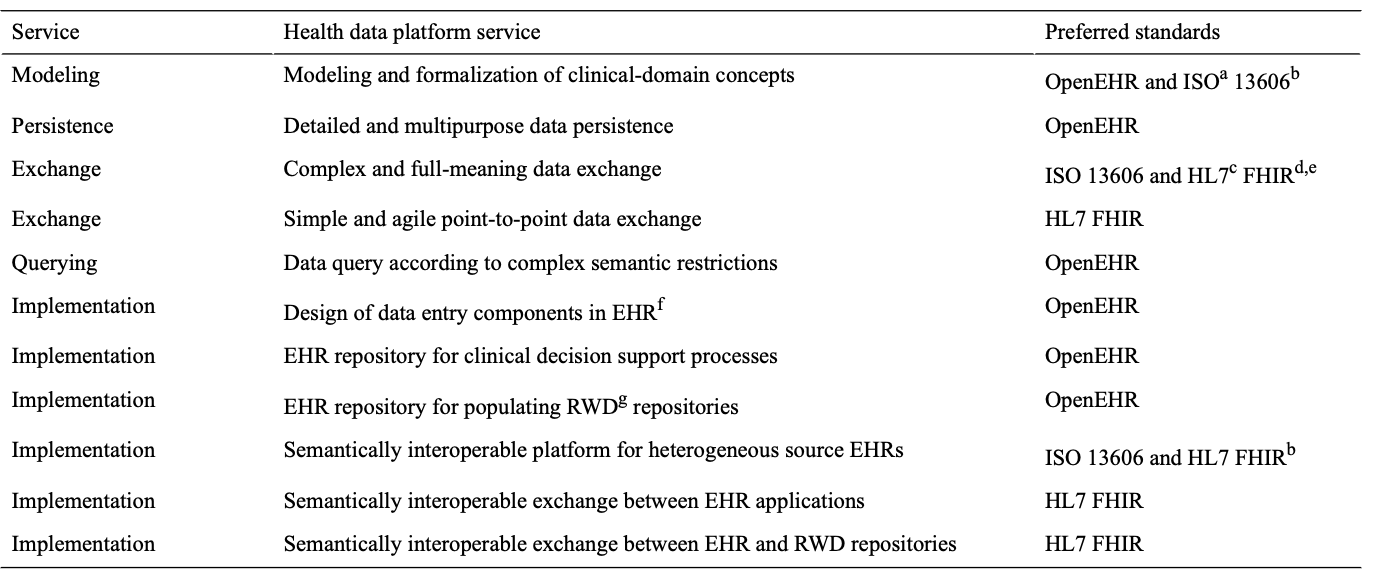
\includegraphics{images/comparison-ehr-standards.png}

}

\end{table}%

For an infectious diseases dataset with a limited scope, OpenEHR, OMOP
and FHIR have been compared and found all to be equally suitable
\citep{rinaldi2021openehr}. Comparing OMOP and FHIR, the latter has been
found to support more granular mappings required for analytics and was
therefore chosen as the standard for the CODA project
\citep{mullie2023coda}.

Although FHIR was originally designed only for exchange between systems,
we propose to use it as the common data model for the design presented
here for the following reasons:

\begin{itemize}
\tightlist
\item
  Industry adoption has significantly increased, as exemplified by
  FHIR-based offering by major cloud providers such as Google, Azure and
  AWS. Also, Africa CDC has explicitly chosen FHIR as the preferred
  standard;
\item
  The widespread availibility of the Bulk FHIR API
  \citep{mandl2020push, jones2021landscape} enables bulk, file-based
  batchwise processing for analytics using the lakehouse architecture as
  detailed in the next section;
\item
  The concept of FHIR Profiles allow localisation to tailor the standard
  to a specific use case. A profile defines rules, extensions, and
  constraints for a resource. We posit that the possible penalty of this
  flexibility, namely having to manage different FHIR versions and/or
  profiles, is less of an issue in the context of LMICs where first
  priority is to exchange datasets such as the International Patient
  Summary (IPS) that are less complex compared to the requirements for
  high income countries;
\item
  Being based on webstandards, the FHIR standard lends itself best for
  further separation of concerns as envisioned by the composable data
  stack. This is an important enabler for the downward scalability of
  the solution;
\item
  With its inherent, graph-like nature, FHIR can be readily incorporated
  into the principles of FAIR data sharing, where FHIR-based data
  repositories can be integrated in an overarching netwerk of FAIR data
  stations \citep{sinaci2023data, pedrera-jimenez2023can}.
\end{itemize}

Possible risks pertaining to the use of FHIR as the common data model,
most notably the possible incompatibilities and/or high costs of
maintenance in supporting different versions, will be addressed in the
Discussion.

\subsection{Open architecture: extending OpenHIE with a composable data
stack}\label{open-architecture-extending-openhie-with-a-composable-data-stack}

\subsubsection{Evolving the data lakehouse to a composable data
stack}\label{evolving-the-data-lakehouse-to-a-composable-data-stack}

Data management and analytics platforms have undergone significant
changes since the first generation of data warehouses were introduced.
Recent studies have shown that the current practice has converged
towards the lakehouse as one of the most commonly used solution designs
\citep{armbrust2021lakehouse, hai2023data, harby2022data}. Lakehouses
typically have a zonal architecture that follow the
Extract-Load-Transform pattern (ELT) where data is ingested from the
source systems in bulk (E), delivered to storage with aligned schemas
(L) and transformed into a format ready for analysis (T)
\citep{hai2023data}. The discerning characteristic of the lakehouse
architecture is its foundation on low-cost and directly-accessible
storage that also provides traditional analytical DBMS management and
performance features such as ACID transactions, data versioning,
auditing, indexing, caching, and query optimization
\citep{armbrust2021lakehouse}. Lakehouses thus combine the key benefits
of data lakes and data warehouses: low-cost storage in an open format
accessible by a variety of systems from the former, and powerful
management and optimization features from the latter.

With respect to current implementations of lakehouse data platforms, we
observe a proliferation of tools with as yet limited standards to
improve technical interoperability. In the analysis of Pedreira et al.
\citep{pedreira2023composable} the requirement for specialization in
data management systems has evolved faster than our software development
practices. This situation has created a siloed landscape composed of
hundreds of products developed and maintained as monoliths, with limited
reuse between systems. It has also affected the end users, who are often
required to learn the idiosyncrasies of dozens of incompatible SQL and
non-SQL API dialects, and settle for systems with incomplete
functionality and inconsistent semantics. To remedy this, Pedreira et
al.~call to (re-)design and implement modern data platforms in terms of
a `composable data stack' as a means to decrease development and
maintenance cost and pick-up the speed of innovation.

While the lakehouse architecture separates the concerns of compute and
storage, the composable data stack takes the separation of concerns is
taken one step further. A composable data system
(Figure~\ref{fig-composable-data-stack}), not only separates the storage
(layer 3) and execution (layer 2), but also separates the user interface
(layer 1) from the execution engine by introducing standards including
Substrait for Intermediate Representation (standard A, IR) and Apache
Arrow for data connectivity and data memory layout (standards B and C,
respectively). The composable data stack can be implemented with current
open source technologies (Figure~\ref{fig-cds-examples}). As an example,
the Ibis user interface is currently sufficiently mature to offer a
standardized dataframe interface to 19 different execution engines.

\begin{figure}

\centering{

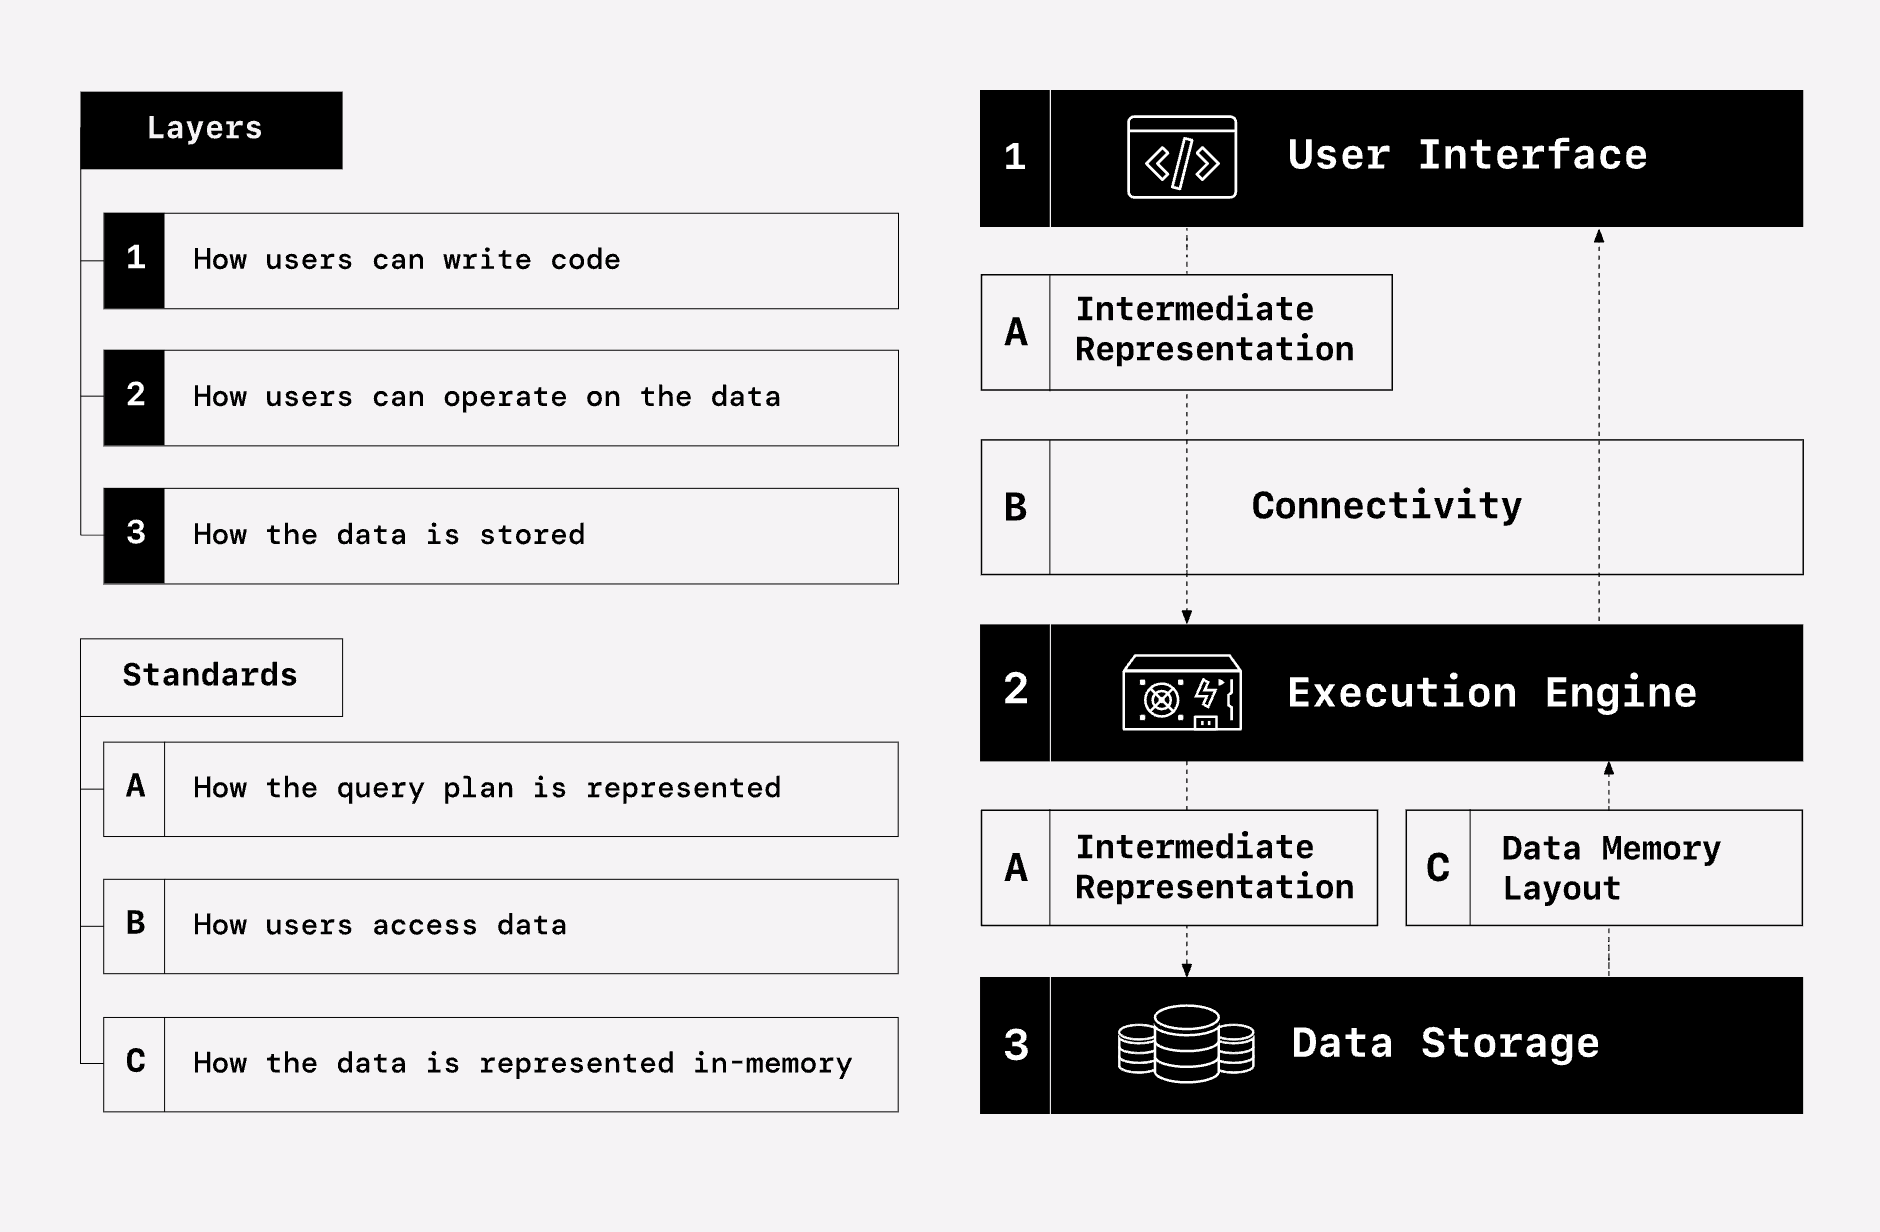
\includegraphics{images/composable-data-stack.png}

}

\caption{\label{fig-composable-data-stack}The composable data stack.
Image source: \url{https://voltrondata.com/codex}.}

\end{figure}%

\begin{figure}

\centering{

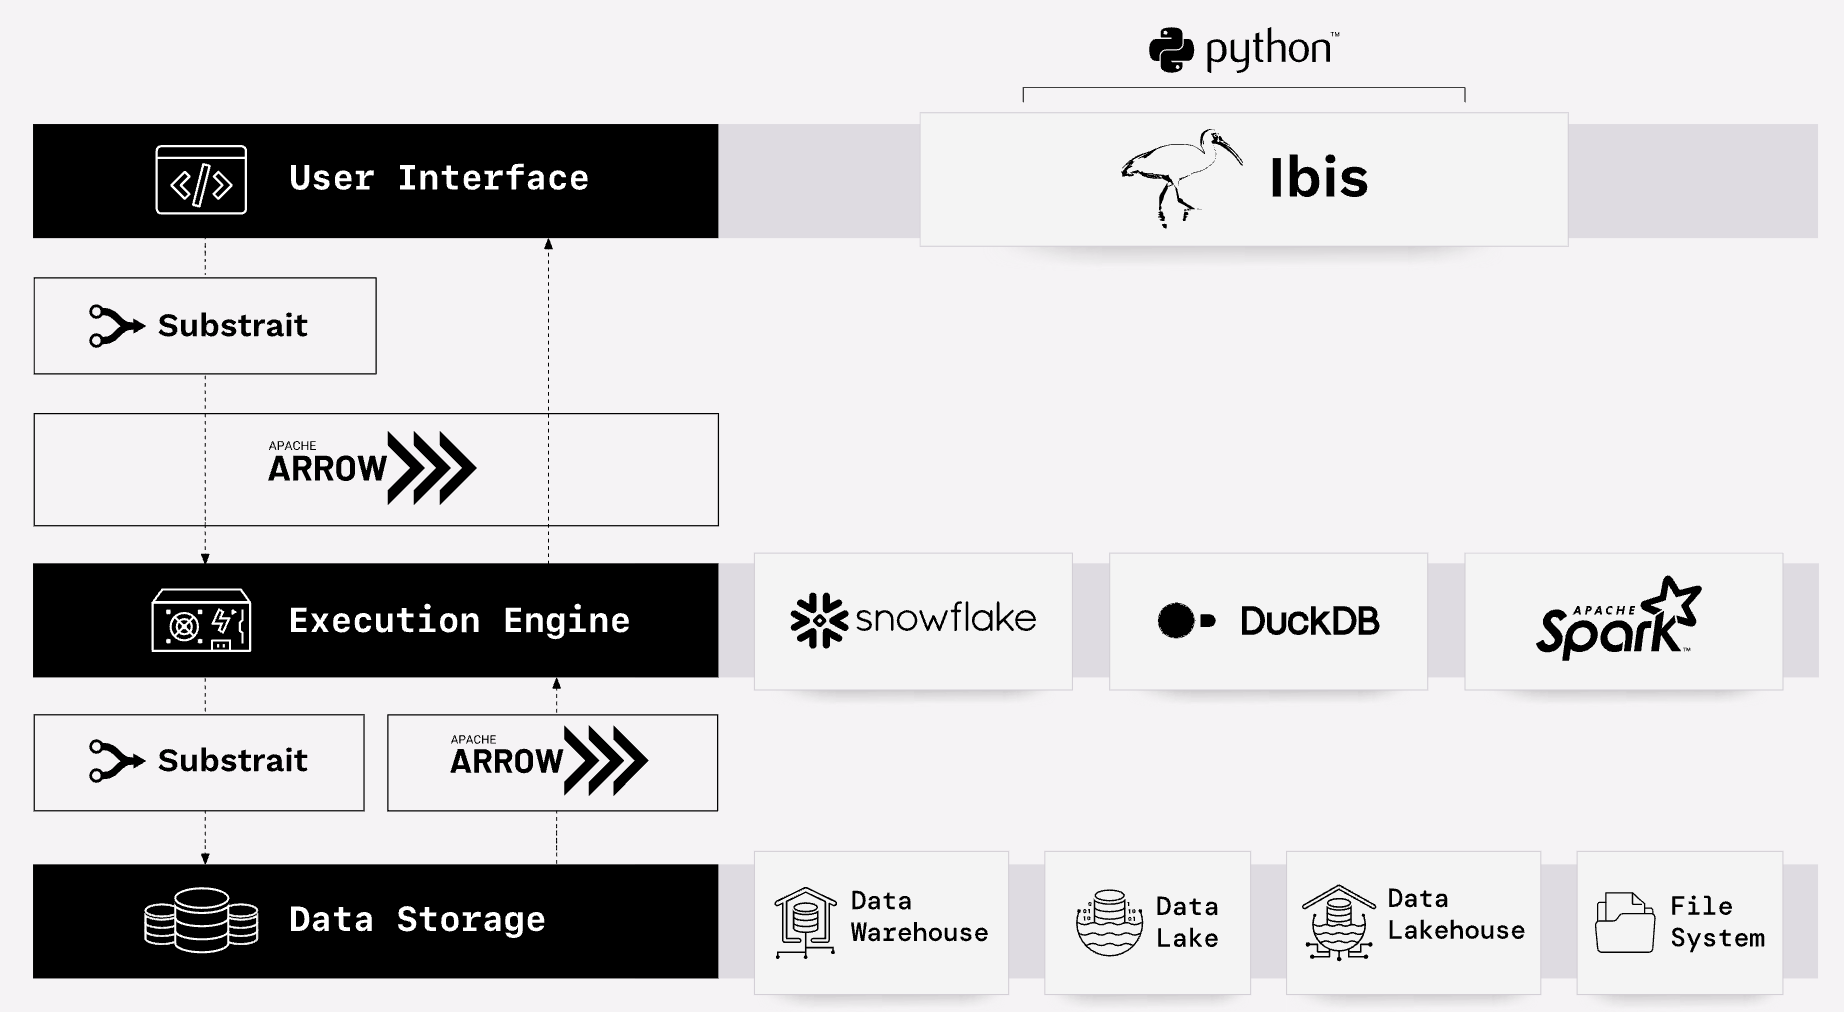
\includegraphics{images/composable-data-stack-implementation-2.png}

}

\caption{\label{fig-cds-examples}Examples of implementations of the
composable data stack. Image source:
\url{https://voltrondata.com/codex}.}

\end{figure}%

\subsubsection{SQL-on-FHIR v2 as an intermediate representation for FHIR
data in tabular
format}\label{sql-on-fhir-v2-as-an-intermediate-representation-for-fhir-data-in-tabular-format}

The premise of separating the user interface from the execution engine
is directly related to the key objective of the SQL-on-FHIR project
(\url{https://build.fhir.org/ig/FHIR/sql-on-fhir-v2/}), namely to make
large-scale analysis of FHIR data accessible to a larger audience,
portable between systems and to make FHIR data work well with the best
available analytic tools, regardless of the technology stack. However,
to use FHIR effectively analysts require a thorough understanding of the
specification as FHIR is represented as a graph of resources, with
detailed semantics defined for references between resources, data types,
terminology, extensions, and many other aspects of the specification.
Most analytic and machine learning use cases require the preparation of
FHIR data using transformations and tabular projections from its
original form. The task of authoring these transformations and
projections is not trivial and there is currently no standard mechanisms
to support reuse.

The solution of the SQL-on-FHIR project is to provide a specification
for defining tabular, use case-specific views of FHIR data. The view
definition and the execution of the view are separated, in such a way
that the definition is portable across systems while the execution
engine (called runners) are system-specific tools or libraries that
apply view definitions to the underlying data layer, optionally making
use of annotations to optimize performance.

\subsubsection{Extending OpenHIE with a FHIR-based composable data
stack}\label{extending-openhie-with-a-fhir-based-composable-data-stack}

We propose to extend the OpenHIE architecture with a ``Data and
Analytics Services'' domain with different service layers by
synthesizing the current best practices of the a lakehouse architecture
of \citep{hai2023data, harby2022data, harby2024data} and the composable
data stack \citep{pedreira2023composable} (Figure~\ref{fig-ohie},
Table~\ref{tbl-data-and-analysis-services}). These 5 services are
considered the core of the FHIR data platform, and although it practice
often a downstream dashboarding or visualization component is used, that
component is not considered part of this architecture as such. NB:
distinction between exploration and dashboarding is not absolute.

\begin{figure}

\centering{

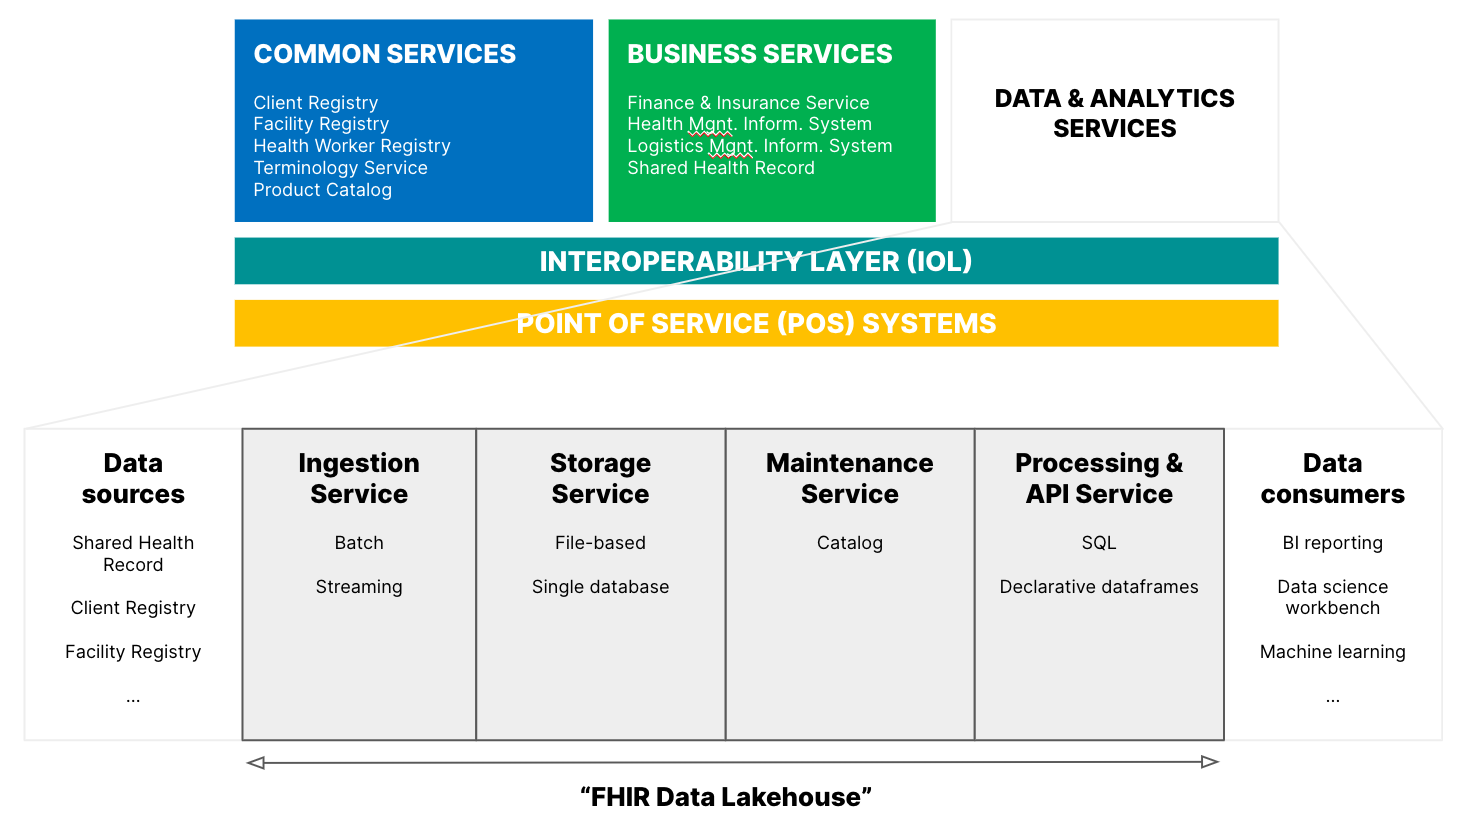
\includegraphics{./images/openhie-extended-architecture.png}

}

\caption{\label{fig-ohie}Proposed extension of the OpenHIE architecture
that includes ``Data and Analytics Services'' as an additional service
domain.}

\end{figure}%

\begin{longtable}[]{@{}
  >{\raggedright\arraybackslash}p{(\columnwidth - 2\tabcolsep) * \real{0.1852}}
  >{\raggedright\arraybackslash}p{(\columnwidth - 2\tabcolsep) * \real{0.8148}}@{}}
\caption{Definition of Data and Analysis
Services}\label{tbl-data-and-analysis-services}\tabularnewline
\toprule\noalign{}
\begin{minipage}[b]{\linewidth}\raggedright
Service
\end{minipage} & \begin{minipage}[b]{\linewidth}\raggedright
Functional requirements
\end{minipage} \\
\midrule\noalign{}
\endfirsthead
\toprule\noalign{}
\begin{minipage}[b]{\linewidth}\raggedright
Service
\end{minipage} & \begin{minipage}[b]{\linewidth}\raggedright
Functional requirements
\end{minipage} \\
\midrule\noalign{}
\endhead
\bottomrule\noalign{}
\endlastfoot
Ingestion & \begin{minipage}[t]{\linewidth}\raggedright
\begin{itemize}
\tightlist
\item
  Bulk
\item
  Streaming
\end{itemize}
\end{minipage} \\
Storage & \begin{minipage}[t]{\linewidth}\raggedright
\begin{itemize}
\tightlist
\item
  File-based blob storage
\item
  Database optimized for online analytical processing (OLAP)
\end{itemize}
\end{minipage} \\
Maintenance & \begin{minipage}[t]{\linewidth}\raggedright
\begin{itemize}
\tightlist
\item
  SQL-on-FHIR View defintions
\item
  Catalog and other maintenance-related functions as defined by Hai et
  al.
\end{itemize}
\end{minipage} \\
Processing \& API & \begin{minipage}[t]{\linewidth}\raggedright
\begin{itemize}
\tightlist
\item
  SQL-on-FHIR Runner
\item
  Execution engine on tabular data as defined in composable data stack
\item
  Capability to participate as a node in federated learning / MPC
  network
\item
  Read-only access to storage
\end{itemize}
\end{minipage} \\
Data Consumer & \begin{minipage}[t]{\linewidth}\raggedright
\begin{itemize}
\tightlist
\item
  SQL interactive development environment (IDE)
\item
  Interactive notebook computing environment \citep{granger2021jupyter}
\item
  BI reporting, dashboarding and data visualization
\end{itemize}
\end{minipage} \\
\end{longtable}

\paragraph{Ingestion}\label{ingestion}

Default workflow is extraction of data from SHR using Bulk FHIR API.
Data contains metadata (incl.~FHIR versions) and fully qualified
semantics, for example, coding systems. Despite this, metadata
extraction and metadata modeling is still required to meet the FAIR
requirements. Issues that need to be solved by these services:

\begin{itemize}
\tightlist
\item
  To prepare for future updates of FHIR versions
\item
  Implement late-binding principle of having increasingly more specific
  FHIR profiles as bulk FHIR data propagates through lakehouse
\end{itemize}

\paragraph{Storage}\label{storage}

\begin{itemize}
\tightlist
\item
  File-based:

  \begin{itemize}
  \tightlist
  \item
    from ndjson to parquet
  \item
    possibly used delta lake for time versioning
  \item
    separation of storage from compute not only for benefits of lower
    TCO, but also be ready for federated learning and MPC in future
  \end{itemize}
\item
  OLAP DBMS

  \begin{itemize}
  \tightlist
  \item
    Often columnar, like Clickhouse and BigQuery
  \item
  \end{itemize}
\end{itemize}

\paragraph{Query \& Processing}\label{query-processing}

\begin{itemize}
\tightlist
\item
  fit in structure of OpenHIE specification
\item
  check which workflows are related to analytics
\item
  Hai calls this `Maintenance'
\end{itemize}

\paragraph{Maintenance}\label{maintenance}

\begin{itemize}
\tightlist
\item
  SQL-on-FHIR Views provide new standard to support mADX aggregate
  reporting
\item
  Maintenance-related functions remain the same
\item
  NB: orchestration falls under data provenance
\end{itemize}

\paragraph{Data consumers}\label{data-consumers}

Strictly speaking not part of the architecture,

\subsection{Open technologies: available digital public
goods}\label{open-technologies-available-digital-public-goods}

Many components of the OpenHIE specification are now available as a
digital public goods. Table~\ref{tbl-digital-public-goods} lists
components that are currently available for implementing the OpenHIE
framework using open source, digital public goods that are compliant
with the FHIR standard, illustrating the maturity of this ecosystem and
development community. With the launch of the Instant OpenHIE
configuration toolkit\citep{InstantOpenHIEv2}, it has become easier to
set up, explore and develop HIEs thereby reducing costs and skills
required for software developers to deploy an OpenHIE architecture for
quicker solution testing and as a starting point for faster production
implementation and customisation. Several frameworks are available that
offer a set of preconfigured components out of the box, such as for
example:

\begin{itemize}
\tightlist
\item
  the ``Open Smart Register Platform'' (OpenSRP), that focuses on
  providing a mobile-first platform, including a FHIR native app
  designed to support the WHO Smart Guidelines
\item
  the OpenHIM Platform, a reference implementation of the Instant
  OpenHIE framework, providing an easy way to set up, manage and operate
  various HIE configurations
\end{itemize}

\begin{table}

\caption{\label{tbl-digital-public-goods}Overview of current open source
implementations of components included in the OpenHIE specification that
are FHIR-compatible. The category Analytics Services is not a part of
the original OpenHIE and is discussed in the paper. Point-of-Service
systems are excluded for brevity. A systematic review of such digital
public goods is beyond the scope of this document.}

\centering{

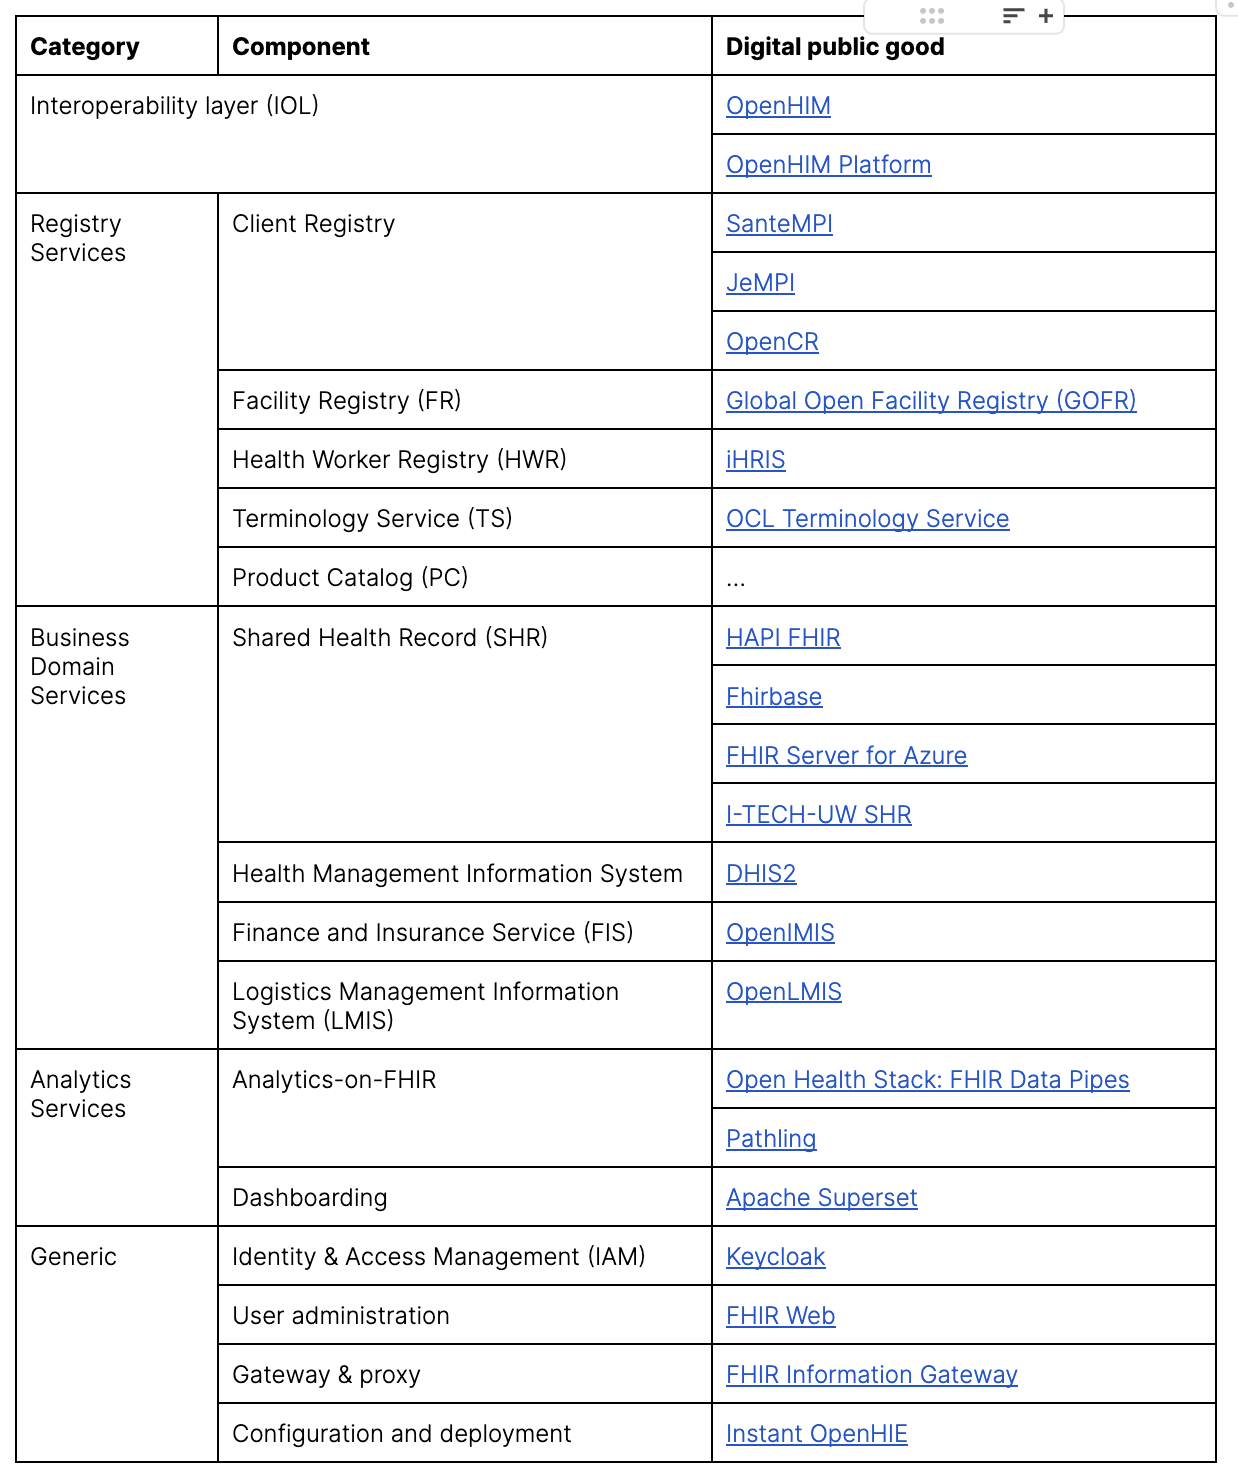
\includegraphics{images/digital-public-goods.png}

}

\end{table}%

Allows for the Data Warehouse data to be visualised via a BI tool
(Apache Superset)

\section{Evaluation}\label{evaluation}

\subsection{OpenHIM platform}\label{openhim-platform}

\begin{itemize}
\tightlist
\item
  One of the most used IOL layers in LMICs. Leading development of
  InstantHIE library to configure OpenHIE infrastructures
\end{itemize}

\url{https://jembi.gitbook.io/openhim-platform/recipes/central-data-repository-with-data-warehousing}

\begin{itemize}
\item
  Accept FHIR bundles submitted securely through an IOL (OpenHIM)
\item
  Stores Clinical FHIR data to a FHIR store (HAPI FHIR)
\item
  Stores Patient Demographic data to an MPI (JeMPI)
\item
  Pushes FHIR resources to Kafka for the reporting pipeline (and other
  systems) to use
\item
  Pulls FHIR data out of Kafka and maps it to flattened tables in the
  Data Warehouse (Clickhouse)
\item
  View generation in different packages, not portable

  \begin{itemize}
  \tightlist
  \item
    Logstash for bulk
  \item
    Kafka for streaming, uses JSON for mappings which looks similar to
    SQL-on-FHIR
  \end{itemize}
\item
\end{itemize}

\subsection{ONA Canopy}\label{ona-canopy}

\subsection{Momcare programme}\label{momcare-programme}

MomCare was launched in Kenya
\citep{huisman2022digital, sanctis2022maintaining} and Tanzania
\citep{shija2021access, mrema2021application} in 2017 and 2019
respectively, with the objective to create transparency on the journeys
of pregnant mothers. The programme is built on three pillars: journey
tracking, quality support and a mobile wallet. MomCare distinguishes two
user groups: mothers are supported during their pregnancy through
reminders and surveys, using SMS as the digital mode of engagement.
Health workers are equipped with an Android-based application, in which
visits, care activities and clinical observations are recorded.
Reimbursements of the maternal clinic are based on the data captured
with SMS and the app, thereby creating a conditional payment scheme,
where providers are partially reimbursed up-front for a fixed bundle of
activities, supplemented by bonus payments based on a predefined set of
care activities.

In its original form, the MomCare programme uses predominantly closed
digital platforms. In Kenya, M-TIBA is the primary digital platform, on
top of which a relatively lightweight custom app has been built as the
engagement layer for the health workers \citep{huisman2022digital}.
M-TIBA provides data access through its data warehouse platform for the
MomCare programme, however, this is not a standardized, general purpose
API. In the case of Tanzania, a stand-alone custom app is used which
does not provide an interface of any kind for interacting with the
platform \citep{mrema2021application}. Given these constraints, to date
the MomCare programme uses a custom-built data warehouse environment as
its main data platform, on which data extractions, transformations and
analysis are performed to generate the operational reports. Feedback
reports for the health workers, in the form of operational dashboards,
are made accessible through the app. Similar reports are provided to the
back-office for the periodic reimbursement to the clinics.

In the periode 2022-2023, a new iteration of MomCare \ldots One of the
practical objectives of the DataCare project was to assess the
complexity and effort required to implement the data transformation
scripts, and reproduce the existing analytic reports. The data was
transformed into 10 FHIR v4 resources as listed in table 1 with the
number of records per resource type. The conceptual data model of the
existing MomCare app could readily be transformed into the FHIR standard
using SQL and validated with a Python library \citep{islam2023fhir}.

The largest challenge during the transformation process pertained to the
absence of unique business identifiers for patients and healthcare
organizations. For patients, either the mobile phone number or the
healthcare insurance number was taken, depending on availability. A
combination of name, address and latitude/longitude coordinates were
used to uniquely identify organizations and locations, as Tanzania does
not have a system in place for this purpose.

The transformed and validated data is uploaded into the FHIR server on a
daily basis using an automated cloud function. Analysis of bulk data was
done by directly reading the standard newline delimited JSON into the
Python pandas data analysis library. Cross checking the output with
queries on the original data confirmed that the whole data pipeline
produced consistent results. For example, the report of the antenatal
coverage metric (number of pregnancies with four or more visits) could
be reproduced per patient journey and aggregated (per year, per
organization etc.) as required for the MomCare reports.

\section{Discussion}\label{discussion}

\subsection{Openness of data
platforms}\label{openness-of-data-platforms}

We specifically address the notion of openness of HDPs in LMICs in terms
of the design-related questions put forward by de Reuver at al.11:

\begin{itemize}
\tightlist
\item
  Object of openness: what data-related resources should data platforms
  make available when opening up (e.g.~data, data products, datadriven
  insights, analytics modules)? Which user groups derive value from
  accessing data-related resources from data platforms (e.g.~data
  providers, data users, intermediaries, developers)?
\item
  Unit of analysis: what is platform-to-platform openness in the context
  of data platforms, given the expectation that different HDPs will
  emerge at various aggregation levels? How do we distinguish
  meta-platforms, forking, and platform interoperability?
\item
  Risk of openness: What are the novel (negative) implications of
  opening up data platforms? How can reflexivity in design help
  providers to resolve the negative implications of openness?
\end{itemize}

\subsection{Comparison with HMIS
component}\label{comparison-with-hmis-component}

\begin{itemize}
\tightlist
\item
  Workflow requirements: Report aggregate data (link): receiver is HMIS,
  mADX
\item
  Functional requirements:
  https://guides.ohie.org/arch-spec/openhie-component-specifications-1/openhie-health-management-information-system-hmis
\end{itemize}

Requirements are similar, but implementation differs: Datamodel is
non-FHIR, focused on DataValue, which conceptually equates to FHIR
Measure

\subsection{The need to a semantic
layer?}\label{the-need-to-a-semantic-layer}

\begin{itemize}
\tightlist
\item
  FHIR and FAIR

  \begin{itemize}
  \tightlist
  \item
    How does FHIR relate to approaches taken by the FAIR community,
    which tend to take more an approach of using knowledge graphs. For
    example, VODAN Africa
    \citep{gebreslassie2023fhir4fair, purnamajati2022data}.
  \item
    FAIR principles vs FHIR graph: is FHIR a FAIR Data Object
  \end{itemize}
\item
  Since we use FHIR, we don't need a semantic layer because that is
  already provided
\item
\end{itemize}

\subsection{Attribute-based access
control}\label{attribute-based-access-control}

\begin{itemize}
\tightlist
\item
  TO DO: if you have generated flattened SQL tables, how are you going
  to manage security?
\item
  Cerbos, attribute based on lineage or anonymized tables
\item
  Catalogs solve this: Tabular.io, Google BigLake. What is open source
  option?
\end{itemize}

\subsection{Federated learning and multiparty
computation}\label{federated-learning-and-multiparty-computation}

\begin{itemize}
\tightlist
\item
  data stations??!
\end{itemize}

\section{Abbreviations}\label{abbreviations}

\begin{longtable}[]{@{}
  >{\raggedright\arraybackslash}p{(\columnwidth - 2\tabcolsep) * \real{0.5000}}
  >{\raggedright\arraybackslash}p{(\columnwidth - 2\tabcolsep) * \real{0.5000}}@{}}
\toprule\noalign{}
\endhead
\bottomrule\noalign{}
\endlastfoot
ELT & Extract, Load and Transform \\
FAIR & Findable, Accessible, Interoperable and Reusable \\
FHIR & Fast Healthcare Interoperability Resources \\
FL & Federated learning \\
HDP & Health data platform, explicitly differentiated from health
digital platform \\
HIE & Health Information Exchange \\
IR & Intermediate Representation \\
LMIC & Low- and middle income countries \\
PET & Privacy-enhancing technologies \\
\end{longtable}


  \bibliography{pharmaccess.bib}


\end{document}
